\documentclass[a4paper,oneside]{memoir}


\usepackage[T2A]{fontenc} % Поддержка русских букв
\usepackage[utf8]{inputenc} % Кодировка utf8
\usepackage[english,russian]{babel}

\usepackage{lipsum}
\usepackage{graphicx} % Required for including pictures

\usepackage{hyperref}
\usepackage{indentfirst}
\usepackage{amsmath}
\usepackage{amssymb}
\usepackage{amsfonts}
\usepackage{float} 
\usepackage{wrapfig}

%\linespread{1.5} % Line spacing

\title{Курс: "Комбинаторика для начинающих".
	
Неделя 7. Контрольная работа.
	 
Выравнивания.}

\newtheorem{task}{Задание}
\newtheorem{solution}{Решение}

 
\author{Александров Алексей, ИУ8-g4}

\date{2020г.}

\begin{document}
	
\maketitle

\begin{task}
Рассмотрим выравнивания слов "росомаха" и "носорог". Сколько всего есть выравниваний длины 9, в которых не выполнено ни условие эквивалентности, ни условие расположения друг над другом символов $ \emptyset $?
\end{task}

\textbf{Ответ:} $ C_9^2 \cdot C_9^1 = 324 $

\begin{solution}
	Выравнивание однозначно определяется тем, как расположены символы $ \emptyset $ в верхней и нижней строчках. В верхней строчке надо выбрать 1 место, в нижней -- 2. Таким образом, общее количество выравниваний равно $ C_9^2 \cdot C_9^1 = 36 \cdot 9 = 324 $.
\end{solution}

\hrulefill

\begin{task}
	Рассмотрим выравнивания слов "росомаха" и "носорог". Сколько всего есть правильных выравниваний (то есть с выполнением двух условий) данных слов?
\end{task}

\textbf{Ответ:} $ C_{15}^7 = C_{15}^8 $

\begin{solution}
	По доказанной теореме количество правильных выравниваний равно $ C_{8+7}^7 = C_{8+7}^8 $, то есть $ C_{15}^7 = C_{15}^8 $.
\end{solution}

\hrulefill

\begin{task}
	Рассмотрим выравнивания слов "росомаха" и "носорог". Какое максимальное количество столбцов может быть в выравнивании?
\end{task}

\textbf{Ответ:} $ 15 $

\begin{solution}
	Так как символы $ \emptyset $ не могут стоять друг над другом, максимальное количество столбцов равно $ 7+8=15 $.
\end{solution}

\hrulefill

\begin{task}
	Рассмотрим выравнивание:
	
	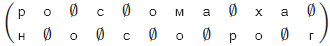
\includegraphics{src/task4}
	
	Сколько выравниваний с ним отождествляется (естественно, мы включаем само это выравнивание)?
\end{task}

\textbf{Ответ:} $ 40 $

\begin{solution}
	Мы можем отождествлять выравнивания, меняя местами столбцы, в которых присутствует $ \emptyset $ в разных строчках. Отсюда ясно, что первый, седьмой и десятый столбцы остаются на месте. Восьмой и девятый, а также одиннадцатый и двенадцатый столбцы мы можем менять местами. Для столбцов со второго по шестой расположение однозначно задаётся верхней строчкой: три непустых и два пустых символа можно выбрать 10 способами. По правилу умножения общее количество выравниваний, эквивалентных данному, равно $  10 \cdot 2 \cdot 2 = 40 $.
\end{solution}

\hrulefill

\begin{task}
	Укажите выравнивания, которые являются одинаковыми (с точки зрения правила отождествления) с выравниванием:
	
		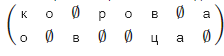
\includegraphics{src/task5}
		
\end{task}

\begin{solution}
	Так как мы можем менять местами только столбцы, то при любом отождествлении первый и седьмой столбцы остаются на месте. Поэтому варианты:
	
			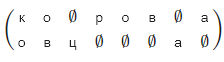
\includegraphics{src/wrong5_1}
			
			и
			
			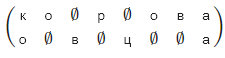
\includegraphics{src/wrong5_2} не подходят.
	
	Оставшиеся два варианта легко получить из имеющихся, используя условие эквивалентности.
	
\end{solution}

\hrulefill

\begin{task}
	Сколько одинаковых подслов содержат слова "росомаха" и "носорог", если каждое подслово считается только один раз? (Подсловом называется последовательность букв слова, расположенных подряд друг за другом. Повторы не учитываются, т.е. если подслово встречается несколько раз, то мы считаем, что одно подслово).
\end{task}

\textbf{Ответ:} $ 7 $

\begin{solution}
	Всего их 7: это подслова "р", "c", "о", "ро", "ос", "осо", "со".
\end{solution}

\hrulefill

\begin{task}
	Сколько одинаковых подслов содержат слова "росомаха" и "носорог"? (Подсловом называется последовательность букв слова, которые расположены подряд друг за другом. Повторы учитываются, т.е. если подслово встречается несколько раз, то мы считаем, что разные подслова).
	
	Примеры: слова "торс" и "трос" содержат следующие общие подслова: "т", "о", "р", "c" - ответ 4; слова "торос" и "трос" содержат следующие общие подслова: "т", "о" (2 раза), "р", "c", "ро", "ос", "рос"- ответ 8.
	
\end{task}

\textbf{Ответ:} $ 12 $

\begin{solution}
	Всего их 12: "р", "о" (6 раз), "c", "ро", "ос", "со", "осо". Буква "o" является общим подсловом $ 6=2\cdot 3 $ раз, т.к. на каждую "верхнюю" букву "o" (которых две в верхнем слове) встречаются три буквы "о" в нижнем слове.
\end{solution}


\end{document}